\documentclass[twoside]{book}

% Packages required by doxygen
\usepackage{fixltx2e}
\usepackage{calc}
\usepackage{doxygen}
\usepackage[export]{adjustbox} % also loads graphicx
\usepackage{graphicx}
\usepackage[utf8]{inputenc}
\usepackage{makeidx}
\usepackage{multicol}
\usepackage{multirow}
\PassOptionsToPackage{warn}{textcomp}
\usepackage{textcomp}
\usepackage[nointegrals]{wasysym}
\usepackage[table]{xcolor}

% Font selection
\usepackage[T1]{fontenc}
\usepackage[scaled=.90]{helvet}
\usepackage{courier}
\usepackage{amssymb}
\usepackage{sectsty}
\renewcommand{\familydefault}{\sfdefault}
\allsectionsfont{%
  \fontseries{bc}\selectfont%
  \color{darkgray}%
}
\renewcommand{\DoxyLabelFont}{%
  \fontseries{bc}\selectfont%
  \color{darkgray}%
}
\newcommand{\+}{\discretionary{\mbox{\scriptsize$\hookleftarrow$}}{}{}}

% Page & text layout
\usepackage{geometry}
\geometry{%
  a4paper,%
  top=2.5cm,%
  bottom=2.5cm,%
  left=2.5cm,%
  right=2.5cm%
}
\tolerance=750
\hfuzz=15pt
\hbadness=750
\setlength{\emergencystretch}{15pt}
\setlength{\parindent}{0cm}
\setlength{\parskip}{0.2cm}
\makeatletter
\renewcommand{\paragraph}{%
  \@startsection{paragraph}{4}{0ex}{-1.0ex}{1.0ex}{%
    \normalfont\normalsize\bfseries\SS@parafont%
  }%
}
\renewcommand{\subparagraph}{%
  \@startsection{subparagraph}{5}{0ex}{-1.0ex}{1.0ex}{%
    \normalfont\normalsize\bfseries\SS@subparafont%
  }%
}
\makeatother

% Headers & footers
\usepackage{fancyhdr}
\pagestyle{fancyplain}
\fancyhead[LE]{\fancyplain{}{\bfseries\thepage}}
\fancyhead[CE]{\fancyplain{}{}}
\fancyhead[RE]{\fancyplain{}{\bfseries\leftmark}}
\fancyhead[LO]{\fancyplain{}{\bfseries\rightmark}}
\fancyhead[CO]{\fancyplain{}{}}
\fancyhead[RO]{\fancyplain{}{\bfseries\thepage}}
\fancyfoot[LE]{\fancyplain{}{}}
\fancyfoot[CE]{\fancyplain{}{}}
\fancyfoot[RE]{\fancyplain{}{\bfseries\scriptsize Generated on Thu Mar 10 2016 14\+:18\+:38 for My Project by Doxygen }}
\fancyfoot[LO]{\fancyplain{}{\bfseries\scriptsize Generated on Thu Mar 10 2016 14\+:18\+:38 for My Project by Doxygen }}
\fancyfoot[CO]{\fancyplain{}{}}
\fancyfoot[RO]{\fancyplain{}{}}
\renewcommand{\footrulewidth}{0.4pt}
\renewcommand{\chaptermark}[1]{%
  \markboth{#1}{}%
}
\renewcommand{\sectionmark}[1]{%
  \markright{\thesection\ #1}%
}

% Indices & bibliography
\usepackage{natbib}
\usepackage[titles]{tocloft}
\setcounter{tocdepth}{3}
\setcounter{secnumdepth}{5}
\makeindex

% Hyperlinks (required, but should be loaded last)
\usepackage{ifpdf}
\ifpdf
  \usepackage[pdftex,pagebackref=true]{hyperref}
\else
  \usepackage[ps2pdf,pagebackref=true]{hyperref}
\fi
\hypersetup{%
  colorlinks=true,%
  linkcolor=blue,%
  citecolor=blue,%
  unicode%
}

% Custom commands
\newcommand{\clearemptydoublepage}{%
  \newpage{\pagestyle{empty}\cleardoublepage}%
}


%===== C O N T E N T S =====

\begin{document}

% Titlepage & ToC
\hypersetup{pageanchor=false,
             bookmarks=true,
             bookmarksnumbered=true,
             pdfencoding=unicode
            }
\pagenumbering{roman}
\begin{titlepage}
\vspace*{7cm}
\begin{center}%
{\Large My Project }\\
\vspace*{1cm}
{\large Generated by Doxygen 1.8.9.1}\\
\vspace*{0.5cm}
{\small Thu Mar 10 2016 14:18:38}\\
\end{center}
\end{titlepage}
\clearemptydoublepage
\tableofcontents
\clearemptydoublepage
\pagenumbering{arabic}
\hypersetup{pageanchor=true}

%--- Begin generated contents ---
\chapter{File Index}
\section{File List}
Here is a list of all documented files with brief descriptions\+:\begin{DoxyCompactList}
\item\contentsline{section}{\hyperlink{algorithm_8h}{algorithm.\+h} \\*Includes three convex hull algorithms It implements Graham scan algorithm, Jarvis march algorithm and Andrew\textquotesingle{}s convex hull algorithm. It also includes cmath library and points header file }{\pageref{algorithm_8h}}{}
\item\contentsline{section}{\hyperlink{animate_8h}{animate.\+h} \\*Displays the working of the algorithms through animation }{\pageref{animate_8h}}{}
\item\contentsline{section}{\hyperlink{createdataset_8cpp}{createdataset.\+cpp} \\*Generates random dataset from a specified distribution }{\pageref{createdataset_8cpp}}{}
\item\contentsline{section}{\hyperlink{driver_8cpp}{driver.\+cpp} \\*Driver program that makes calls to Covex Hull A\+P\+I }{\pageref{driver_8cpp}}{}
\item\contentsline{section}{\hyperlink{points_8h}{points.\+h} \\*Provides an abstract representation of a point and a set of points. It provides all the functions to manipulate points to perform various operations required by the Convex hull algorithms }{\pageref{points_8h}}{}
\end{DoxyCompactList}

\chapter{File Documentation}
\hypertarget{algorithm_8h}{}\section{algorithm.\+h File Reference}
\label{algorithm_8h}\index{algorithm.\+h@{algorithm.\+h}}


Includes three convex hull algorithms It implements Graham scan algorithm, Jarvis march algorithm and Andrew\textquotesingle{}s convex hull algorithm. It also includes cmath library and points header file.  


{\ttfamily \#include $<$algorithm$>$}\\*
{\ttfamily \#include $<$cmath$>$}\\*
{\ttfamily \#include \char`\"{}animate.\+h\char`\"{}}\\*
Include dependency graph for algorithm.\+h\+:

\hypertarget{animate_8h}{}\section{animate.\+h File Reference}
\label{animate_8h}\index{animate.\+h@{animate.\+h}}


Displays the working of the algorithms through animation.  


{\ttfamily \#include \char`\"{}points.\+h\char`\"{}}\\*
Include dependency graph for animate.\+h\+:
% FIG 0
This graph shows which files directly or indirectly include this file\+:
% FIG 1
\subsection*{Macros}
\begin{DoxyCompactItemize}
\item 
\hypertarget{animate_8h_a241aeeb764887ae5e3de58b98f04b16d}{}\#define \hyperlink{animate_8h_a241aeeb764887ae5e3de58b98f04b16d}{W\+I\+D\+T\+H}~60\label{animate_8h_a241aeeb764887ae5e3de58b98f04b16d}

\begin{DoxyCompactList}\small\item\em Width of the Clipping plane is 60. \end{DoxyCompactList}\item 
\hypertarget{animate_8h_aed89bd71aee8be823e8a20ec4e093c1e}{}\#define \hyperlink{animate_8h_aed89bd71aee8be823e8a20ec4e093c1e}{H\+E\+I\+G\+H\+T}~60\label{animate_8h_aed89bd71aee8be823e8a20ec4e093c1e}

\begin{DoxyCompactList}\small\item\em Height of the Clipping plane is 60. \end{DoxyCompactList}\item 
\hypertarget{animate_8h_a4af1b6159e447ba72652bb7fcdfa726e}{}\#define \hyperlink{animate_8h_a4af1b6159e447ba72652bb7fcdfa726e}{E\+S\+C}~27\label{animate_8h_a4af1b6159e447ba72652bb7fcdfa726e}

\begin{DoxyCompactList}\small\item\em Exit the G\+L window. \end{DoxyCompactList}\item 
\hypertarget{animate_8h_a03dcc6d12ab68f4c3dd8faf2ed1dbc79}{}\#define \hyperlink{animate_8h_a03dcc6d12ab68f4c3dd8faf2ed1dbc79}{M\+U\+\_\+\+S\+E\+C}~1000\label{animate_8h_a03dcc6d12ab68f4c3dd8faf2ed1dbc79}

\begin{DoxyCompactList}\small\item\em Multiplier for microseconds. \end{DoxyCompactList}\end{DoxyCompactItemize}
\subsection*{Functions}
\begin{DoxyCompactItemize}
\item 
void \hyperlink{animate_8h_a5f7658bbd8ecc54af8d77b14f68dabd4}{process\+Normal\+Keys} (unsigned char key, int xx, int yy)
\begin{DoxyCompactList}\small\item\em Event handler for a key press. \end{DoxyCompactList}\item 
\hypertarget{animate_8h_af1d8945a7d8f56dedd1c3dc2b7528217}{}void \hyperlink{animate_8h_af1d8945a7d8f56dedd1c3dc2b7528217}{graphics\+Initialize} ()\label{animate_8h_af1d8945a7d8f56dedd1c3dc2b7528217}

\begin{DoxyCompactList}\small\item\em Initializes viewing graphics parameters and registers callbacks. \end{DoxyCompactList}\item 
void \hyperlink{animate_8h_a164b8cbd9f06eaa4af7bd878087199e6}{draw\+Point} (\hyperlink{points_8h_a7bff2da864fb642dcbfa06bc2ac74fa7}{point} a)
\begin{DoxyCompactList}\small\item\em Draws a point on the G\+L window. \end{DoxyCompactList}\item 
void \hyperlink{animate_8h_a3f1a3c82f580d30650114baa50f5658e}{plot\+Points} (\hyperlink{points_8h_a4bb5da68740936bfcd019aa4e0483431}{pointset} \hyperlink{points_8h_a96bcafe6a15c3e350f400c283f410192}{S})
\begin{DoxyCompactList}\small\item\em Plots the set of points on G\+L window. \end{DoxyCompactList}\item 
void \hyperlink{animate_8h_a00e7dc2a5b11639762d1bae6e6bdf4fe}{draw\+Line} (\hyperlink{points_8h_a7bff2da864fb642dcbfa06bc2ac74fa7}{point} a, \hyperlink{points_8h_a7bff2da864fb642dcbfa06bc2ac74fa7}{point} b)
\begin{DoxyCompactList}\small\item\em Draws a line segment between two given points. \end{DoxyCompactList}\item 
void \hyperlink{animate_8h_aecd9aa84d3fe76fe2c5c209b5dd23f67}{draw\+Line\+Loop} (\hyperlink{points_8h_a4bb5da68740936bfcd019aa4e0483431}{pointset} \hyperlink{points_8h_a96bcafe6a15c3e350f400c283f410192}{S})
\begin{DoxyCompactList}\small\item\em Draws a closed loop of line segments. \end{DoxyCompactList}\item 
void \hyperlink{animate_8h_a8947dcec1b8d99e0df2f4bc686ba2a13}{draw\+Poly\+Line} (\hyperlink{points_8h_a4bb5da68740936bfcd019aa4e0483431}{pointset} \hyperlink{points_8h_a96bcafe6a15c3e350f400c283f410192}{S})
\begin{DoxyCompactList}\small\item\em Draws a polyline. \end{DoxyCompactList}\item 
void \hyperlink{animate_8h_a5d4b4187d67900909e9b0f8e7dcb0fe5}{draw\+Poly\+Line} (\hyperlink{points_8h_aaf29cda67857ebaa72fbb96c0457c700}{pointstack} \hyperlink{points_8h_a96bcafe6a15c3e350f400c283f410192}{S})
\begin{DoxyCompactList}\small\item\em Converts pointstack to pointset and draws a polyline. \end{DoxyCompactList}\item 
void \hyperlink{animate_8h_a970847358ec151f53ebc4a27bd753572}{animate\+Selection} (\hyperlink{points_8h_a4bb5da68740936bfcd019aa4e0483431}{pointset} \hyperlink{points_8h_a9fa54c2e52b99276ec2a7ddf634874fc}{C\+H}, \hyperlink{points_8h_a7bff2da864fb642dcbfa06bc2ac74fa7}{point} a, \hyperlink{points_8h_a7bff2da864fb642dcbfa06bc2ac74fa7}{point} b)
\begin{DoxyCompactList}\small\item\em Initializes the frame parameters. Draws current portion of convex hull and the point being considered. \end{DoxyCompactList}\item 
void \hyperlink{animate_8h_ad0b7b5229b04149b36b3b5235236ae76}{animate\+Selection} (\hyperlink{points_8h_aaf29cda67857ebaa72fbb96c0457c700}{pointstack} \hyperlink{points_8h_a9fa54c2e52b99276ec2a7ddf634874fc}{C\+H}, \hyperlink{points_8h_a7bff2da864fb642dcbfa06bc2ac74fa7}{point} a, \hyperlink{points_8h_a7bff2da864fb642dcbfa06bc2ac74fa7}{point} b, \hyperlink{points_8h_a7bff2da864fb642dcbfa06bc2ac74fa7}{point} c, \hyperlink{points_8h_aaf29cda67857ebaa72fbb96c0457c700}{pointstack} C\+H2)
\begin{DoxyCompactList}\small\item\em Initializes the frame parameters. Draws current portion of convex hull and the point being considered. \end{DoxyCompactList}\item 
void \hyperlink{animate_8h_ad5468108be9f9f84342d9e2c2811fe56}{draw\+Convex\+Hull} (\hyperlink{points_8h_a4bb5da68740936bfcd019aa4e0483431}{pointset} \hyperlink{points_8h_a9fa54c2e52b99276ec2a7ddf634874fc}{C\+H})
\begin{DoxyCompactList}\small\item\em Refreshes the G\+L window and draws the final convex hull. \end{DoxyCompactList}\end{DoxyCompactItemize}
\subsection*{Variables}
\begin{DoxyCompactItemize}
\item 
int \hyperlink{animate_8h_a95a13658ced0801ed2e2d349bd150dc0}{animtog} = 0
\end{DoxyCompactItemize}


\subsection{Detailed Description}
Displays the working of the algorithms through animation. 



\subsection{Function Documentation}
\hypertarget{animate_8h_a970847358ec151f53ebc4a27bd753572}{}\index{animate.\+h@{animate.\+h}!animate\+Selection@{animate\+Selection}}
\index{animate\+Selection@{animate\+Selection}!animate.\+h@{animate.\+h}}
\subsubsection[{animate\+Selection}]{\setlength{\rightskip}{0pt plus 5cm}void animate\+Selection (
\begin{DoxyParamCaption}
\item[{{\bf pointset}}]{C\+H, }
\item[{{\bf point}}]{a, }
\item[{{\bf point}}]{b}
\end{DoxyParamCaption}
)}\label{animate_8h_a970847358ec151f53ebc4a27bd753572}


Initializes the frame parameters. Draws current portion of convex hull and the point being considered. 


\begin{DoxyParams}{Parameters}
{\em C\+H} & current portion of convex hull. \\
\hline
{\em a} & terminal point of current segment. \\
\hline
{\em b} & terminal point of current segment. \\
\hline
\end{DoxyParams}

\begin{DoxyCode}
148 \{
149     glClear(GL\_COLOR\_BUFFER\_BIT | GL\_DEPTH\_BUFFER\_BIT);
150 
151     \hyperlink{animate_8h_a3f1a3c82f580d30650114baa50f5658e}{plotPoints}( \hyperlink{points_8h_a96bcafe6a15c3e350f400c283f410192}{S} );
152 
153     glColor3f(0.0, 1.0, 0.0);
154     \hyperlink{animate_8h_a8947dcec1b8d99e0df2f4bc686ba2a13}{drawPolyLine}( \hyperlink{points_8h_a9fa54c2e52b99276ec2a7ddf634874fc}{CH} );
155 
156     glColor3f(1.0, 0.0, 0.0);
157     \hyperlink{animate_8h_a00e7dc2a5b11639762d1bae6e6bdf4fe}{drawLine}( a, b );
158 
159     glutSwapBuffers();
160     usleep( (1000/\hyperlink{points_8h_a96bcafe6a15c3e350f400c283f410192}{S}.size())* \hyperlink{animate_8h_a03dcc6d12ab68f4c3dd8faf2ed1dbc79}{MU\_SEC} );
161 \}
\end{DoxyCode}
\hypertarget{animate_8h_ad0b7b5229b04149b36b3b5235236ae76}{}\index{animate.\+h@{animate.\+h}!animate\+Selection@{animate\+Selection}}
\index{animate\+Selection@{animate\+Selection}!animate.\+h@{animate.\+h}}
\subsubsection[{animate\+Selection}]{\setlength{\rightskip}{0pt plus 5cm}void animate\+Selection (
\begin{DoxyParamCaption}
\item[{{\bf pointstack}}]{C\+H, }
\item[{{\bf point}}]{a, }
\item[{{\bf point}}]{b, }
\item[{{\bf point}}]{c, }
\item[{{\bf pointstack}}]{C\+H2}
\end{DoxyParamCaption}
)}\label{animate_8h_ad0b7b5229b04149b36b3b5235236ae76}


Initializes the frame parameters. Draws current portion of convex hull and the point being considered. 


\begin{DoxyParams}{Parameters}
{\em C\+H} & current portion of convex hull. \\
\hline
{\em a} & terminal point of current segment. \\
\hline
{\em b} & terminal point of current segment. \\
\hline
{\em c} & terminal point of current segment. \\
\hline
{\em C\+H2} & previous portion of convex hull. Used only for Andrew\textquotesingle{}s algorithm. \\
\hline
\end{DoxyParams}

\begin{DoxyCode}
172 \{
173     glClear(GL\_COLOR\_BUFFER\_BIT | GL\_DEPTH\_BUFFER\_BIT);
174 
175     \hyperlink{animate_8h_a3f1a3c82f580d30650114baa50f5658e}{plotPoints}( \hyperlink{points_8h_a96bcafe6a15c3e350f400c283f410192}{S} );
176 
177     glColor3f(0.0, 1.0, 0.0);
178     \hyperlink{animate_8h_a8947dcec1b8d99e0df2f4bc686ba2a13}{drawPolyLine}( \hyperlink{points_8h_a9fa54c2e52b99276ec2a7ddf634874fc}{CH} );
179     \hyperlink{animate_8h_a8947dcec1b8d99e0df2f4bc686ba2a13}{drawPolyLine}( CH2 );
180 
181     glColor3f(1.0, 0.0, 0.0);
182     \hyperlink{animate_8h_a00e7dc2a5b11639762d1bae6e6bdf4fe}{drawLine}( a, b );
183     glColor3f(0.0, 0.0, 1.0);
184     \hyperlink{animate_8h_a00e7dc2a5b11639762d1bae6e6bdf4fe}{drawLine}( b, c );
185 
186     glutSwapBuffers();
187     usleep( (10000/\hyperlink{points_8h_a96bcafe6a15c3e350f400c283f410192}{S}.size()) * \hyperlink{animate_8h_a03dcc6d12ab68f4c3dd8faf2ed1dbc79}{MU\_SEC} );
188 \}
\end{DoxyCode}
\hypertarget{animate_8h_ad5468108be9f9f84342d9e2c2811fe56}{}\index{animate.\+h@{animate.\+h}!draw\+Convex\+Hull@{draw\+Convex\+Hull}}
\index{draw\+Convex\+Hull@{draw\+Convex\+Hull}!animate.\+h@{animate.\+h}}
\subsubsection[{draw\+Convex\+Hull}]{\setlength{\rightskip}{0pt plus 5cm}void draw\+Convex\+Hull (
\begin{DoxyParamCaption}
\item[{{\bf pointset}}]{C\+H}
\end{DoxyParamCaption}
)}\label{animate_8h_ad5468108be9f9f84342d9e2c2811fe56}


Refreshes the G\+L window and draws the final convex hull. 


\begin{DoxyParams}{Parameters}
{\em C\+H} & pointset containing final convex hull. \\
\hline
\end{DoxyParams}

\begin{DoxyCode}
195 \{
196     glClear(GL\_COLOR\_BUFFER\_BIT | GL\_DEPTH\_BUFFER\_BIT);
197 
198     \hyperlink{animate_8h_a3f1a3c82f580d30650114baa50f5658e}{plotPoints}( \hyperlink{points_8h_a96bcafe6a15c3e350f400c283f410192}{S} );
199 
200     glColor3f(0.0, 1.0, 0.0);
201     \hyperlink{animate_8h_aecd9aa84d3fe76fe2c5c209b5dd23f67}{drawLineLoop}( \hyperlink{points_8h_a9fa54c2e52b99276ec2a7ddf634874fc}{CH} );
202 \}\end{DoxyCode}
\hypertarget{animate_8h_a00e7dc2a5b11639762d1bae6e6bdf4fe}{}\index{animate.\+h@{animate.\+h}!draw\+Line@{draw\+Line}}
\index{draw\+Line@{draw\+Line}!animate.\+h@{animate.\+h}}
\subsubsection[{draw\+Line}]{\setlength{\rightskip}{0pt plus 5cm}void draw\+Line (
\begin{DoxyParamCaption}
\item[{{\bf point}}]{a, }
\item[{{\bf point}}]{b}
\end{DoxyParamCaption}
)}\label{animate_8h_a00e7dc2a5b11639762d1bae6e6bdf4fe}


Draws a line segment between two given points. 


\begin{DoxyParams}{Parameters}
{\em a} & Terminal point of segment. \\
\hline
{\em a} & Terminal point of segment. \\
\hline
\end{DoxyParams}

\begin{DoxyCode}
89 \{
90     glBegin(GL\_LINES);
91         glVertex3f( a.first, a.second, 0.0f );
92         glVertex3f( b.first, b.second, 0.0f );
93     glEnd();
94 \}
\end{DoxyCode}
\hypertarget{animate_8h_aecd9aa84d3fe76fe2c5c209b5dd23f67}{}\index{animate.\+h@{animate.\+h}!draw\+Line\+Loop@{draw\+Line\+Loop}}
\index{draw\+Line\+Loop@{draw\+Line\+Loop}!animate.\+h@{animate.\+h}}
\subsubsection[{draw\+Line\+Loop}]{\setlength{\rightskip}{0pt plus 5cm}void draw\+Line\+Loop (
\begin{DoxyParamCaption}
\item[{{\bf pointset}}]{S}
\end{DoxyParamCaption}
)}\label{animate_8h_aecd9aa84d3fe76fe2c5c209b5dd23f67}


Draws a closed loop of line segments. 


\begin{DoxyParams}{Parameters}
{\em S} & Ordered pointset. \\
\hline
\end{DoxyParams}

\begin{DoxyCode}
101 \{
102     glBegin(GL\_LINE\_LOOP);
103         \textcolor{keywordflow}{for} ( \textcolor{keywordtype}{int} i = 0; i < \hyperlink{points_8h_a96bcafe6a15c3e350f400c283f410192}{S}.size(); i++ )
104         \{
105             glVertex3f( \hyperlink{points_8h_a96bcafe6a15c3e350f400c283f410192}{S}[i].first, \hyperlink{points_8h_a96bcafe6a15c3e350f400c283f410192}{S}[i].second, 0.0f );
106         \}
107     glEnd();
108 \}
\end{DoxyCode}
\hypertarget{animate_8h_a164b8cbd9f06eaa4af7bd878087199e6}{}\index{animate.\+h@{animate.\+h}!draw\+Point@{draw\+Point}}
\index{draw\+Point@{draw\+Point}!animate.\+h@{animate.\+h}}
\subsubsection[{draw\+Point}]{\setlength{\rightskip}{0pt plus 5cm}void draw\+Point (
\begin{DoxyParamCaption}
\item[{{\bf point}}]{a}
\end{DoxyParamCaption}
)}\label{animate_8h_a164b8cbd9f06eaa4af7bd878087199e6}


Draws a point on the G\+L window. 


\begin{DoxyParams}{Parameters}
{\em a} & Coordinates of point to be drawn. \\
\hline
\end{DoxyParams}

\begin{DoxyCode}
64 \{
65     glBegin(GL\_POINTS);
66         glVertex3f( a.first, a.second, 0.0f );
67     glEnd();
68 \}
\end{DoxyCode}
\hypertarget{animate_8h_a8947dcec1b8d99e0df2f4bc686ba2a13}{}\index{animate.\+h@{animate.\+h}!draw\+Poly\+Line@{draw\+Poly\+Line}}
\index{draw\+Poly\+Line@{draw\+Poly\+Line}!animate.\+h@{animate.\+h}}
\subsubsection[{draw\+Poly\+Line}]{\setlength{\rightskip}{0pt plus 5cm}void draw\+Poly\+Line (
\begin{DoxyParamCaption}
\item[{{\bf pointset}}]{S}
\end{DoxyParamCaption}
)}\label{animate_8h_a8947dcec1b8d99e0df2f4bc686ba2a13}


Draws a polyline. 


\begin{DoxyParams}{Parameters}
{\em S} & Ordered pointset. \\
\hline
\end{DoxyParams}

\begin{DoxyCode}
115 \{
116     glBegin(GL\_LINES);
117         \textcolor{keywordflow}{for} ( \textcolor{keywordtype}{int} i = 1; i < \hyperlink{points_8h_a96bcafe6a15c3e350f400c283f410192}{S}.size(); i++ )
118         \{
119             glVertex3f( \hyperlink{points_8h_a96bcafe6a15c3e350f400c283f410192}{S}[i].first, \hyperlink{points_8h_a96bcafe6a15c3e350f400c283f410192}{S}[i].second, 0.0f );
120             glVertex3f( \hyperlink{points_8h_a96bcafe6a15c3e350f400c283f410192}{S}[i-1].first, \hyperlink{points_8h_a96bcafe6a15c3e350f400c283f410192}{S}[i-1].second, 0.0f );
121         \}
122     glEnd();
123 \}
\end{DoxyCode}
\hypertarget{animate_8h_a5d4b4187d67900909e9b0f8e7dcb0fe5}{}\index{animate.\+h@{animate.\+h}!draw\+Poly\+Line@{draw\+Poly\+Line}}
\index{draw\+Poly\+Line@{draw\+Poly\+Line}!animate.\+h@{animate.\+h}}
\subsubsection[{draw\+Poly\+Line}]{\setlength{\rightskip}{0pt plus 5cm}void draw\+Poly\+Line (
\begin{DoxyParamCaption}
\item[{{\bf pointstack}}]{S}
\end{DoxyParamCaption}
)}\label{animate_8h_a5d4b4187d67900909e9b0f8e7dcb0fe5}


Converts pointstack to pointset and draws a polyline. 


\begin{DoxyParams}{Parameters}
{\em S} & Ordered pointstack. \\
\hline
\end{DoxyParams}

\begin{DoxyCode}
130 \{
131     \hyperlink{points_8h_a4bb5da68740936bfcd019aa4e0483431}{pointset} T;
132     \textcolor{keywordflow}{while}( !\hyperlink{points_8h_a96bcafe6a15c3e350f400c283f410192}{S}.empty() )
133     \{
134         T.addPoint( \hyperlink{points_8h_a96bcafe6a15c3e350f400c283f410192}{S}.top() );
135         \hyperlink{points_8h_a96bcafe6a15c3e350f400c283f410192}{S}.pop();
136     \}
137 
138     \hyperlink{animate_8h_a8947dcec1b8d99e0df2f4bc686ba2a13}{drawPolyLine}( T );
139 \}
\end{DoxyCode}
\hypertarget{animate_8h_a3f1a3c82f580d30650114baa50f5658e}{}\index{animate.\+h@{animate.\+h}!plot\+Points@{plot\+Points}}
\index{plot\+Points@{plot\+Points}!animate.\+h@{animate.\+h}}
\subsubsection[{plot\+Points}]{\setlength{\rightskip}{0pt plus 5cm}void plot\+Points (
\begin{DoxyParamCaption}
\item[{{\bf pointset}}]{S}
\end{DoxyParamCaption}
)}\label{animate_8h_a3f1a3c82f580d30650114baa50f5658e}


Plots the set of points on G\+L window. 


\begin{DoxyParams}{Parameters}
{\em S} & Pointset to be drawn. \\
\hline
\end{DoxyParams}

\begin{DoxyCode}
75 \{
76     glColor3f( 1.0, 1.0, 0.0 );
77     \textcolor{keywordflow}{for} ( \textcolor{keywordtype}{int} i = 0; i < \hyperlink{points_8h_a96bcafe6a15c3e350f400c283f410192}{S}.size(); i++ )
78     \{
79         \hyperlink{animate_8h_a164b8cbd9f06eaa4af7bd878087199e6}{drawPoint}( \hyperlink{points_8h_a96bcafe6a15c3e350f400c283f410192}{S}[i] );
80     \}
81 \}
\end{DoxyCode}
\hypertarget{animate_8h_a5f7658bbd8ecc54af8d77b14f68dabd4}{}\index{animate.\+h@{animate.\+h}!process\+Normal\+Keys@{process\+Normal\+Keys}}
\index{process\+Normal\+Keys@{process\+Normal\+Keys}!animate.\+h@{animate.\+h}}
\subsubsection[{process\+Normal\+Keys}]{\setlength{\rightskip}{0pt plus 5cm}void process\+Normal\+Keys (
\begin{DoxyParamCaption}
\item[{unsigned char}]{key, }
\item[{int}]{xx, }
\item[{int}]{yy}
\end{DoxyParamCaption}
)}\label{animate_8h_a5f7658bbd8ecc54af8d77b14f68dabd4}


Event handler for a key press. 


\begin{DoxyParams}{Parameters}
{\em key} & Key pressed. \\
\hline
{\em xx} & Standard G\+L variable. \\
\hline
{\em yy} & Standard G\+L variable. \\
\hline
\end{DoxyParams}

\begin{DoxyCode}
39 \{   
40     \textcolor{keywordflow}{if}( key == \hyperlink{animate_8h_a4af1b6159e447ba72652bb7fcdfa726e}{ESC} )
41         exit(0);
42 \}
\end{DoxyCode}


\subsection{Variable Documentation}
\hypertarget{animate_8h_a95a13658ced0801ed2e2d349bd150dc0}{}\index{animate.\+h@{animate.\+h}!animtog@{animtog}}
\index{animtog@{animtog}!animate.\+h@{animate.\+h}}
\subsubsection[{animtog}]{\setlength{\rightskip}{0pt plus 5cm}int animtog = 0}\label{animate_8h_a95a13658ced0801ed2e2d349bd150dc0}
Animation toggle variable. 
\hypertarget{createdataset_8cpp}{}\section{createdataset.\+cpp File Reference}
\label{createdataset_8cpp}\index{createdataset.\+cpp@{createdataset.\+cpp}}


Generates random dataset from a specified distribution.  


{\ttfamily \#include $<$stdio.\+h$>$}\\*
{\ttfamily \#include $<$bits/stdc++.\+h$>$}\\*
{\ttfamily \#include $<$stdlib.\+h$>$}\\*
{\ttfamily \#include $<$iostream$>$}\\*
{\ttfamily \#include $<$random$>$}\\*
Include dependency graph for createdataset.\+cpp\+:
% FIG 0
\subsection*{Functions}
\begin{DoxyCompactItemize}
\item 
\hypertarget{createdataset_8cpp_ae66f6b31b5ad750f1fe042a706a4e3d4}{}int {\bfseries main} ()\label{createdataset_8cpp_ae66f6b31b5ad750f1fe042a706a4e3d4}

\end{DoxyCompactItemize}


\subsection{Detailed Description}
Generates random dataset from a specified distribution. 


\hypertarget{driver_8cpp}{}\section{/home/aditya/gitfolder/personal/assignments/\+Computational Geometry/driver.cpp File Reference}
\label{driver_8cpp}\index{/home/aditya/gitfolder/personal/assignments/\+Computational Geometry/driver.\+cpp@{/home/aditya/gitfolder/personal/assignments/\+Computational Geometry/driver.\+cpp}}


Driver program that makes calls to Covex Hull A\+P\+I.  


{\ttfamily \#include $<$iostream$>$}\\*
{\ttfamily \#include $<$cstdio$>$}\\*
{\ttfamily \#include $<$unistd.\+h$>$}\\*
{\ttfamily \#include $<$bits/stdc++.\+h$>$}\\*
{\ttfamily \#include $<$G\+L/glut.\+h$>$}\\*
{\ttfamily \#include \char`\"{}cgal/algorithm.\+h\char`\"{}}\\*
Include dependency graph for driver.\+cpp\+:\nopagebreak
\begin{figure}[H]
\begin{center}
\leavevmode
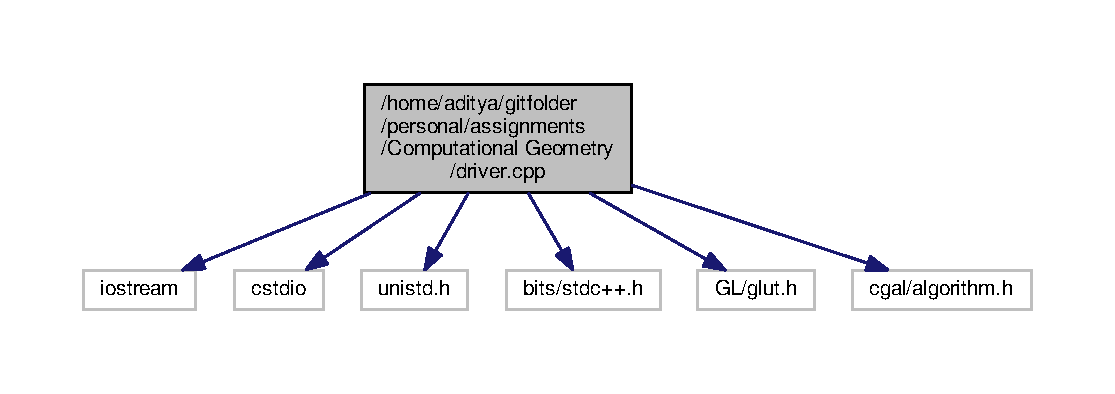
\includegraphics[width=350pt]{driver_8cpp__incl}
\end{center}
\end{figure}
\subsection*{Functions}
\begin{DoxyCompactItemize}
\item 
\hypertarget{driver_8cpp_a91c42686f3245f22fb6b17ba5372d92c}{}void \hyperlink{driver_8cpp_a91c42686f3245f22fb6b17ba5372d92c}{render\+Scene} ()\label{driver_8cpp_a91c42686f3245f22fb6b17ba5372d92c}

\begin{DoxyCompactList}\small\item\em Registered call back for G\+L display function. \end{DoxyCompactList}\item 
int \hyperlink{driver_8cpp_a0ddf1224851353fc92bfbff6f499fa97}{main} (int argc, char $\ast$argv\mbox{[}$\,$\mbox{]})
\begin{DoxyCompactList}\small\item\em Main function. \end{DoxyCompactList}\end{DoxyCompactItemize}


\subsection{Detailed Description}
Driver program that makes calls to Covex Hull A\+P\+I. 



\subsection{Function Documentation}
\hypertarget{driver_8cpp_a0ddf1224851353fc92bfbff6f499fa97}{}\index{driver.\+cpp@{driver.\+cpp}!main@{main}}
\index{main@{main}!driver.\+cpp@{driver.\+cpp}}
\subsubsection[{main}]{\setlength{\rightskip}{0pt plus 5cm}int main (
\begin{DoxyParamCaption}
\item[{int}]{argc, }
\item[{char $\ast$}]{argv\mbox{[}$\,$\mbox{]}}
\end{DoxyParamCaption}
)}\label{driver_8cpp_a0ddf1224851353fc92bfbff6f499fa97}


Main function. 


\begin{DoxyParams}{Parameters}
{\em argc} & default commandline argument. \\
\hline
{\em argv} & default commandline arguments. \\
\hline
\end{DoxyParams}

\begin{DoxyCode}
44 \{
45 
46     cin >> size >> animtog;
47     \textcolor{keywordflow}{for} ( \textcolor{keywordtype}{int} i = 0; i < size; i++ )
48     \{
49         \textcolor{keywordtype}{double} x, y;
50         cin >> x >> y;
51         S.addPoint( coord(x, y) );
52     \}
53 
54     glutInit(&argc, argv);
55     graphicsInitialize();
56     glutDisplayFunc( \hyperlink{driver_8cpp_a91c42686f3245f22fb6b17ba5372d92c}{renderScene} );
57     glutMainLoop();
58 
59     \textcolor{keywordflow}{return} 0;
60 \}
\end{DoxyCode}

\hypertarget{points_8h}{}\section{points.\+h File Reference}
\label{points_8h}\index{points.\+h@{points.\+h}}


Provides an abstract representation of a point and a set of points. It provides all the functions to manipulate points to perform various operations required by the Convex hull algorithms.  


{\ttfamily \#include $<$vector$>$}\\*
{\ttfamily \#include $<$stack$>$}\\*
{\ttfamily \#include $<$cmath$>$}\\*
Include dependency graph for points.\+h\+:
% FIG 0
This graph shows which files directly or indirectly include this file\+:
% FIG 1
\subsection*{Macros}
\begin{DoxyCompactItemize}
\item 
\hypertarget{points_8h_a7bff2da864fb642dcbfa06bc2ac74fa7}{}\#define \hyperlink{points_8h_a7bff2da864fb642dcbfa06bc2ac74fa7}{point}~pair$<$double, double$>$\label{points_8h_a7bff2da864fb642dcbfa06bc2ac74fa7}

\begin{DoxyCompactList}\small\item\em Pair of x, y coordinate of a point. \end{DoxyCompactList}\item 
\hypertarget{points_8h_a4bb5da68740936bfcd019aa4e0483431}{}\#define \hyperlink{points_8h_a4bb5da68740936bfcd019aa4e0483431}{pointset}~vector$<$\hyperlink{points_8h_a7bff2da864fb642dcbfa06bc2ac74fa7}{point}$>$\label{points_8h_a4bb5da68740936bfcd019aa4e0483431}

\begin{DoxyCompactList}\small\item\em Vector containing all the points. \end{DoxyCompactList}\item 
\hypertarget{points_8h_aaf29cda67857ebaa72fbb96c0457c700}{}\#define \hyperlink{points_8h_aaf29cda67857ebaa72fbb96c0457c700}{pointstack}~stack$<$\hyperlink{points_8h_a7bff2da864fb642dcbfa06bc2ac74fa7}{point}$>$\label{points_8h_aaf29cda67857ebaa72fbb96c0457c700}

\begin{DoxyCompactList}\small\item\em Stack of given points. \end{DoxyCompactList}\item 
\hypertarget{points_8h_ace6dc239253765056895d916f3b2c1a3}{}\#define \hyperlink{points_8h_ace6dc239253765056895d916f3b2c1a3}{coord}~make\+\_\+pair\label{points_8h_ace6dc239253765056895d916f3b2c1a3}

\begin{DoxyCompactList}\small\item\em a macro to call make\+\_\+pair function. \end{DoxyCompactList}\item 
\hypertarget{points_8h_aa822716f3e615cf7dbf531b9bd54751f}{}\#define \hyperlink{points_8h_aa822716f3e615cf7dbf531b9bd54751f}{add\+Point}~push\+\_\+back\label{points_8h_aa822716f3e615cf7dbf531b9bd54751f}

\begin{DoxyCompactList}\small\item\em a macro to call push\+\_\+back function. \end{DoxyCompactList}\item 
\hypertarget{points_8h_a0f48c17c99b7b74c0d8e10cc7dec387c}{}\#define \hyperlink{points_8h_a0f48c17c99b7b74c0d8e10cc7dec387c}{del\+Point}~pop\+\_\+back\label{points_8h_a0f48c17c99b7b74c0d8e10cc7dec387c}

\begin{DoxyCompactList}\small\item\em a macro to call pop\+\_\+back function. \end{DoxyCompactList}\item 
\hypertarget{points_8h_adf770fe2eec438e3758ffe905dbae208}{}\#define \hyperlink{points_8h_adf770fe2eec438e3758ffe905dbae208}{I\+N\+V\+A\+L\+I\+D}~777\label{points_8h_adf770fe2eec438e3758ffe905dbae208}

\begin{DoxyCompactList}\small\item\em Term used to declare a point as invalid. \end{DoxyCompactList}\item 
\#define \hyperlink{points_8h_a598a3330b3c21701223ee0ca14316eca}{P\+I}~3.\+141592653589793
\begin{DoxyCompactList}\small\item\em A macro that replaces the value of P\+I with 3.\+141592653589793. \end{DoxyCompactList}\item 
\hypertarget{points_8h_ac328e551bde3d39b6d7b8cc9e048d941}{}\#define \hyperlink{points_8h_ac328e551bde3d39b6d7b8cc9e048d941}{Z\+E\+R\+O}~0.\+0f\label{points_8h_ac328e551bde3d39b6d7b8cc9e048d941}

\begin{DoxyCompactList}\small\item\em Term used to represent Zero angle in float. \end{DoxyCompactList}\end{DoxyCompactItemize}
\subsection*{Functions}
\begin{DoxyCompactItemize}
\item 
void \hyperlink{points_8h_a069a8f32f68b6f6bc2c283aa6ba08b7d}{print\+Point} (\hyperlink{points_8h_a7bff2da864fb642dcbfa06bc2ac74fa7}{point} a)
\begin{DoxyCompactList}\small\item\em Prints a point ( its x and y coordinate). \end{DoxyCompactList}\item 
double \hyperlink{points_8h_a0c8e9f0ed435ed6d8bc9e5a1f7a34d41}{dist\+Between} (\hyperlink{points_8h_a7bff2da864fb642dcbfa06bc2ac74fa7}{point} a, \hyperlink{points_8h_a7bff2da864fb642dcbfa06bc2ac74fa7}{point} b)
\begin{DoxyCompactList}\small\item\em Calculates the distance between two points passed as parameters. \end{DoxyCompactList}\item 
double \hyperlink{points_8h_a11aeb88925b4b67d19896322ded98d95}{angle\+Between} (\hyperlink{points_8h_a7bff2da864fb642dcbfa06bc2ac74fa7}{point} a, \hyperlink{points_8h_a7bff2da864fb642dcbfa06bc2ac74fa7}{point} b, \hyperlink{points_8h_a7bff2da864fb642dcbfa06bc2ac74fa7}{point} c)
\begin{DoxyCompactList}\small\item\em Calculates the angle between two points wrt third point passed as parameters using cos. \end{DoxyCompactList}\item 
int \hyperlink{points_8h_aa610aa9018fc7e42689297d64344038c}{signed\+Area} (\hyperlink{points_8h_a7bff2da864fb642dcbfa06bc2ac74fa7}{point} a, \hyperlink{points_8h_a7bff2da864fb642dcbfa06bc2ac74fa7}{point} b, \hyperlink{points_8h_a7bff2da864fb642dcbfa06bc2ac74fa7}{point} c)
\begin{DoxyCompactList}\small\item\em Calculates the signed area of three points to find the direction in which these three points connect to each other. \end{DoxyCompactList}\item 
\hyperlink{points_8h_a7bff2da864fb642dcbfa06bc2ac74fa7}{point} \hyperlink{points_8h_ade0ea07172344151e5797441f4102e4a}{get\+Interior\+Point} (\hyperlink{points_8h_a4bb5da68740936bfcd019aa4e0483431}{pointset} \hyperlink{points_8h_a96bcafe6a15c3e350f400c283f410192}{S})
\begin{DoxyCompactList}\small\item\em Finds a point lying inside the convex hull. Used for Graham scan. \end{DoxyCompactList}\item 
\hyperlink{points_8h_a7bff2da864fb642dcbfa06bc2ac74fa7}{point} \hyperlink{points_8h_a6f23edf4476103596aa762acc72a5b3e}{get\+Exterior\+Point} (\hyperlink{points_8h_a4bb5da68740936bfcd019aa4e0483431}{pointset} \hyperlink{points_8h_a96bcafe6a15c3e350f400c283f410192}{S})
\begin{DoxyCompactList}\small\item\em Finds a point lying outside the convex hull. Used for Jarvis March and Andrew\textquotesingle{}s algorithm. \end{DoxyCompactList}\item 
int \hyperlink{points_8h_aa09466518aeb7b0b12b5729c5af6f6c1}{search\+Point\+Set} (\hyperlink{points_8h_a4bb5da68740936bfcd019aa4e0483431}{pointset} \hyperlink{points_8h_a96bcafe6a15c3e350f400c283f410192}{S}, \hyperlink{points_8h_a7bff2da864fb642dcbfa06bc2ac74fa7}{point} a)
\begin{DoxyCompactList}\small\item\em Checks if a given point is one among the given set of points. \end{DoxyCompactList}\item 
bool \hyperlink{points_8h_ad7f985653af831e1bb1fa671f5b9e0ed}{check\+Right\+Turn} (\hyperlink{points_8h_a7bff2da864fb642dcbfa06bc2ac74fa7}{point} a, \hyperlink{points_8h_a7bff2da864fb642dcbfa06bc2ac74fa7}{point} b, \hyperlink{points_8h_a7bff2da864fb642dcbfa06bc2ac74fa7}{point} c)
\begin{DoxyCompactList}\small\item\em Finds if a set of points in a sequence make a right turn or not. Used in Graham scan and Andrew\textquotesingle{}s algorithm. \end{DoxyCompactList}\item 
void \hyperlink{points_8h_a2ded54db967c9115b1ce31f9c83de60b}{print\+Convex\+Hull} (\hyperlink{points_8h_a4bb5da68740936bfcd019aa4e0483431}{pointset} \hyperlink{points_8h_a9fa54c2e52b99276ec2a7ddf634874fc}{C\+H})
\begin{DoxyCompactList}\small\item\em Prints the points lying on the Convex Hull via S\+T\+D\+O\+U\+T. \end{DoxyCompactList}\end{DoxyCompactItemize}
\subsection*{Variables}
\begin{DoxyCompactItemize}
\item 
int \hyperlink{points_8h_a439227feff9d7f55384e8780cfc2eb82}{size} = 0
\item 
int \hyperlink{points_8h_ab221478ca7d05e317e8f2f5d8d1697d0}{size\+C\+H} = 0
\item 
\hyperlink{points_8h_a4bb5da68740936bfcd019aa4e0483431}{pointset} \hyperlink{points_8h_a96bcafe6a15c3e350f400c283f410192}{S}
\item 
\hyperlink{points_8h_a4bb5da68740936bfcd019aa4e0483431}{pointset} \hyperlink{points_8h_a9fa54c2e52b99276ec2a7ddf634874fc}{C\+H}
\item 
\hyperlink{points_8h_aaf29cda67857ebaa72fbb96c0457c700}{pointstack} \hyperlink{points_8h_aad7054d73665bb0329acd163521d7c65}{E\+T}
\end{DoxyCompactItemize}


\subsection{Detailed Description}
Provides an abstract representation of a point and a set of points. It provides all the functions to manipulate points to perform various operations required by the Convex hull algorithms. 



\subsection{Macro Definition Documentation}
\hypertarget{points_8h_a598a3330b3c21701223ee0ca14316eca}{}\index{points.\+h@{points.\+h}!P\+I@{P\+I}}
\index{P\+I@{P\+I}!points.\+h@{points.\+h}}
\subsubsection[{P\+I}]{\setlength{\rightskip}{0pt plus 5cm}\#define P\+I~3.\+141592653589793}\label{points_8h_a598a3330b3c21701223ee0ca14316eca}


A macro that replaces the value of P\+I with 3.\+141592653589793. 

Term used to represent P\+I for angle calculation measured in radians. 

\subsection{Function Documentation}
\hypertarget{points_8h_a11aeb88925b4b67d19896322ded98d95}{}\index{points.\+h@{points.\+h}!angle\+Between@{angle\+Between}}
\index{angle\+Between@{angle\+Between}!points.\+h@{points.\+h}}
\subsubsection[{angle\+Between}]{\setlength{\rightskip}{0pt plus 5cm}double angle\+Between (
\begin{DoxyParamCaption}
\item[{{\bf point}}]{a, }
\item[{{\bf point}}]{b, }
\item[{{\bf point}}]{c}
\end{DoxyParamCaption}
)}\label{points_8h_a11aeb88925b4b67d19896322ded98d95}


Calculates the angle between two points wrt third point passed as parameters using cos. 


\begin{DoxyParams}{Parameters}
{\em a} & First point. \\
\hline
{\em c} & Second point. \\
\hline
{\em b} & Reference point. \\
\hline
\end{DoxyParams}

\begin{DoxyCode}
127 \{
128     \textcolor{comment}{/*A local variable. Declares and initializes angle between points as 0. */}
129     \textcolor{keywordtype}{double} angle = 0;   
130 
131     \textcolor{comment}{/*  A local variable. Determines the distance between point 1 and reference point. */}
132     \textcolor{keywordtype}{double} moda = \hyperlink{points_8h_a0c8e9f0ed435ed6d8bc9e5a1f7a34d41}{distBetween}(a, b); 
133     
134     \textcolor{comment}{/*  A local variable. Determines the distance between point 2 and reference point. */}
135     \textcolor{keywordtype}{double} modb = \hyperlink{points_8h_a0c8e9f0ed435ed6d8bc9e5a1f7a34d41}{distBetween}(c, b);     
136 
137     \textcolor{keywordflow}{if} ( moda == 0 or modb == 0)
138     \{
139         \textcolor{keywordflow}{return} \hyperlink{points_8h_adf770fe2eec438e3758ffe905dbae208}{INVALID};
140     \}
141 
142     \textcolor{comment}{/*  A local variable. Calculates the dot product between the segments ac and bc. */}
143     \textcolor{keywordtype}{double} dot; 
144     dot = ((a.first - b.first) * (c.first - b.first)) + ((a.second - b.second) * (c.second - b.second));
145 
146     angle = acos(dot / (moda * modb));
147     
148     \textcolor{keywordflow}{return} angle;
149 \}
\end{DoxyCode}
\hypertarget{points_8h_ad7f985653af831e1bb1fa671f5b9e0ed}{}\index{points.\+h@{points.\+h}!check\+Right\+Turn@{check\+Right\+Turn}}
\index{check\+Right\+Turn@{check\+Right\+Turn}!points.\+h@{points.\+h}}
\subsubsection[{check\+Right\+Turn}]{\setlength{\rightskip}{0pt plus 5cm}bool check\+Right\+Turn (
\begin{DoxyParamCaption}
\item[{{\bf point}}]{a, }
\item[{{\bf point}}]{b, }
\item[{{\bf point}}]{c}
\end{DoxyParamCaption}
)}\label{points_8h_ad7f985653af831e1bb1fa671f5b9e0ed}


Finds if a set of points in a sequence make a right turn or not. Used in Graham scan and Andrew\textquotesingle{}s algorithm. 


\begin{DoxyParams}{Parameters}
{\em a} & First point. \\
\hline
{\em b} & Second point. \\
\hline
{\em c} & Third point. \\
\hline
\end{DoxyParams}

\begin{DoxyCode}
244 \{
245     \textcolor{keywordflow}{if} ( \hyperlink{points_8h_aa610aa9018fc7e42689297d64344038c}{signedArea}( a, b, c ) > 0 )
246         \textcolor{keywordflow}{return} \textcolor{keyword}{false};
247     \textcolor{keywordflow}{else}
248         \textcolor{keywordflow}{return} \textcolor{keyword}{true};
249 \}
\end{DoxyCode}
\hypertarget{points_8h_a0c8e9f0ed435ed6d8bc9e5a1f7a34d41}{}\index{points.\+h@{points.\+h}!dist\+Between@{dist\+Between}}
\index{dist\+Between@{dist\+Between}!points.\+h@{points.\+h}}
\subsubsection[{dist\+Between}]{\setlength{\rightskip}{0pt plus 5cm}double dist\+Between (
\begin{DoxyParamCaption}
\item[{{\bf point}}]{a, }
\item[{{\bf point}}]{b}
\end{DoxyParamCaption}
)}\label{points_8h_a0c8e9f0ed435ed6d8bc9e5a1f7a34d41}


Calculates the distance between two points passed as parameters. 


\begin{DoxyParams}{Parameters}
{\em a} & First point. \\
\hline
{\em b} & Second point. \\
\hline
\end{DoxyParams}

\begin{DoxyCode}
105 \{
106     \textcolor{comment}{/* A local variable. Declares and initializes distance as 0. */}
107     \textcolor{keywordtype}{double} distance = 0;    
108     
109     \textcolor{comment}{/* A local variable. Determines squared distance in x direction. */}
110     \textcolor{keywordtype}{double} x = (a.first - b.first) * (a.first - b.first);   
111     
112     \textcolor{comment}{/* A local variable. Determines squared distance in y direction. */}
113     \textcolor{keywordtype}{double} y = (a.second - b.second) * (a.second - b.second);   
114     
115     distance = sqrt( x + y );
116         
117     \textcolor{keywordflow}{return} distance;
118 \}
\end{DoxyCode}
\hypertarget{points_8h_a6f23edf4476103596aa762acc72a5b3e}{}\index{points.\+h@{points.\+h}!get\+Exterior\+Point@{get\+Exterior\+Point}}
\index{get\+Exterior\+Point@{get\+Exterior\+Point}!points.\+h@{points.\+h}}
\subsubsection[{get\+Exterior\+Point}]{\setlength{\rightskip}{0pt plus 5cm}{\bf point} get\+Exterior\+Point (
\begin{DoxyParamCaption}
\item[{{\bf pointset}}]{S}
\end{DoxyParamCaption}
)}\label{points_8h_a6f23edf4476103596aa762acc72a5b3e}


Finds a point lying outside the convex hull. Used for Jarvis March and Andrew\textquotesingle{}s algorithm. 


\begin{DoxyParams}{Parameters}
{\em S} & Set of points to find the interior point within. \\
\hline
\end{DoxyParams}

\begin{DoxyCode}
204 \{
205     \textcolor{comment}{/* A local variable. Declares and initializes the outside point as the first point in pointset and
       later assigns it a point with minimum y coordiante value. */}
206     \hyperlink{points_8h_a7bff2da864fb642dcbfa06bc2ac74fa7}{point} outside = \hyperlink{points_8h_a96bcafe6a15c3e350f400c283f410192}{S}[0]; 
207     \textcolor{comment}{//printPoint( outside );}
208 
209     \textcolor{keywordflow}{for} ( \textcolor{keywordtype}{int} i = 1; i < \hyperlink{points_8h_a96bcafe6a15c3e350f400c283f410192}{S}.size(); i++ )
210     \{
211         \textcolor{keywordflow}{if} ( \hyperlink{points_8h_a96bcafe6a15c3e350f400c283f410192}{S}[i].second < outside.second )
212         \{
213             outside = \hyperlink{points_8h_a96bcafe6a15c3e350f400c283f410192}{S}[i];
214         \}
215     \}
216 
217     \textcolor{keywordflow}{return} outside;
218 \}
\end{DoxyCode}
\hypertarget{points_8h_ade0ea07172344151e5797441f4102e4a}{}\index{points.\+h@{points.\+h}!get\+Interior\+Point@{get\+Interior\+Point}}
\index{get\+Interior\+Point@{get\+Interior\+Point}!points.\+h@{points.\+h}}
\subsubsection[{get\+Interior\+Point}]{\setlength{\rightskip}{0pt plus 5cm}{\bf point} get\+Interior\+Point (
\begin{DoxyParamCaption}
\item[{{\bf pointset}}]{S}
\end{DoxyParamCaption}
)}\label{points_8h_ade0ea07172344151e5797441f4102e4a}


Finds a point lying inside the convex hull. Used for Graham scan. 


\begin{DoxyParams}{Parameters}
{\em S} & Set of points to find the interior point within. \\
\hline
\end{DoxyParams}

\begin{DoxyCode}
179 \{
180     \textcolor{keywordtype}{int} i = 3;
181     
182     \textcolor{comment}{/* A local variable. Declares and initializes the inside point as (0,0). */}
183     \hyperlink{points_8h_a7bff2da864fb642dcbfa06bc2ac74fa7}{point} inside = \hyperlink{points_8h_ace6dc239253765056895d916f3b2c1a3}{coord}(0, 0);   
184     \hyperlink{points_8h_a7bff2da864fb642dcbfa06bc2ac74fa7}{point} a = \hyperlink{points_8h_a96bcafe6a15c3e350f400c283f410192}{S}[0];
185     \hyperlink{points_8h_a7bff2da864fb642dcbfa06bc2ac74fa7}{point} b = \hyperlink{points_8h_a96bcafe6a15c3e350f400c283f410192}{S}[1];
186     \hyperlink{points_8h_a7bff2da864fb642dcbfa06bc2ac74fa7}{point} c = \hyperlink{points_8h_a96bcafe6a15c3e350f400c283f410192}{S}[2];
187 
188     \textcolor{keywordflow}{while}( \hyperlink{points_8h_aa610aa9018fc7e42689297d64344038c}{signedArea}(a, b, c) == 0 )
189     \{
190         b = c;
191         c = \hyperlink{points_8h_a96bcafe6a15c3e350f400c283f410192}{S}[i++];
192     \}
193     
194     \textcolor{comment}{//finds a centroid of three non-collinear points and makes it the interior point.}
195     inside = \hyperlink{points_8h_ace6dc239253765056895d916f3b2c1a3}{coord}((a.first + b.first + c.first)/3, (a.second + b.second + c.second)/3);
196     \textcolor{keywordflow}{return} inside;
197 \}
\end{DoxyCode}
\hypertarget{points_8h_a2ded54db967c9115b1ce31f9c83de60b}{}\index{points.\+h@{points.\+h}!print\+Convex\+Hull@{print\+Convex\+Hull}}
\index{print\+Convex\+Hull@{print\+Convex\+Hull}!points.\+h@{points.\+h}}
\subsubsection[{print\+Convex\+Hull}]{\setlength{\rightskip}{0pt plus 5cm}void print\+Convex\+Hull (
\begin{DoxyParamCaption}
\item[{{\bf pointset}}]{C\+H}
\end{DoxyParamCaption}
)}\label{points_8h_a2ded54db967c9115b1ce31f9c83de60b}


Prints the points lying on the Convex Hull via S\+T\+D\+O\+U\+T. 


\begin{DoxyParams}{Parameters}
{\em C\+H} & pointset \\
\hline
\end{DoxyParams}

\begin{DoxyCode}
256 \{
257     cout << \hyperlink{points_8h_a9fa54c2e52b99276ec2a7ddf634874fc}{CH}.size() << endl;
258     \textcolor{keywordflow}{for}( \textcolor{keywordtype}{int} i = 0; i < \hyperlink{points_8h_a9fa54c2e52b99276ec2a7ddf634874fc}{CH}.size() ; i++)
259     \{
260         \hyperlink{points_8h_a069a8f32f68b6f6bc2c283aa6ba08b7d}{printPoint}( \hyperlink{points_8h_a9fa54c2e52b99276ec2a7ddf634874fc}{CH}[i] );
261     \}
262 \}
\end{DoxyCode}
\hypertarget{points_8h_a069a8f32f68b6f6bc2c283aa6ba08b7d}{}\index{points.\+h@{points.\+h}!print\+Point@{print\+Point}}
\index{print\+Point@{print\+Point}!points.\+h@{points.\+h}}
\subsubsection[{print\+Point}]{\setlength{\rightskip}{0pt plus 5cm}void print\+Point (
\begin{DoxyParamCaption}
\item[{{\bf point}}]{a}
\end{DoxyParamCaption}
)}\label{points_8h_a069a8f32f68b6f6bc2c283aa6ba08b7d}


Prints a point ( its x and y coordinate). 


\begin{DoxyParams}{Parameters}
{\em a} & A point. \\
\hline
\end{DoxyParams}

\begin{DoxyCode}
95 \{
96     cout << setprecision(9) << (double)a.first << \textcolor{stringliteral}{" "} << (\textcolor{keywordtype}{double})a.second << endl;
97 \}
\end{DoxyCode}
\hypertarget{points_8h_aa09466518aeb7b0b12b5729c5af6f6c1}{}\index{points.\+h@{points.\+h}!search\+Point\+Set@{search\+Point\+Set}}
\index{search\+Point\+Set@{search\+Point\+Set}!points.\+h@{points.\+h}}
\subsubsection[{search\+Point\+Set}]{\setlength{\rightskip}{0pt plus 5cm}int search\+Point\+Set (
\begin{DoxyParamCaption}
\item[{{\bf pointset}}]{S, }
\item[{{\bf point}}]{a}
\end{DoxyParamCaption}
)}\label{points_8h_aa09466518aeb7b0b12b5729c5af6f6c1}


Checks if a given point is one among the given set of points. 


\begin{DoxyParams}{Parameters}
{\em S} & Set of points.. \\
\hline
{\em a} & A point to be searched. Returns 1 if the point belongs to the pointset else returns -\/1. \\
\hline
\end{DoxyParams}

\begin{DoxyCode}
227 \{
228     \textcolor{keywordflow}{for} ( \textcolor{keywordtype}{int} i = 0; i < \hyperlink{points_8h_a96bcafe6a15c3e350f400c283f410192}{S}.size(); i++ )
229     \{
230         \textcolor{keywordflow}{if} ( \hyperlink{points_8h_a96bcafe6a15c3e350f400c283f410192}{S}[i].first == a.first and \hyperlink{points_8h_a96bcafe6a15c3e350f400c283f410192}{S}[i].second == a.second )
231             \textcolor{keywordflow}{return} i;
232     \}
233 
234     \textcolor{keywordflow}{return} -1;
235 \}
\end{DoxyCode}
\hypertarget{points_8h_aa610aa9018fc7e42689297d64344038c}{}\index{points.\+h@{points.\+h}!signed\+Area@{signed\+Area}}
\index{signed\+Area@{signed\+Area}!points.\+h@{points.\+h}}
\subsubsection[{signed\+Area}]{\setlength{\rightskip}{0pt plus 5cm}int signed\+Area (
\begin{DoxyParamCaption}
\item[{{\bf point}}]{a, }
\item[{{\bf point}}]{b, }
\item[{{\bf point}}]{c}
\end{DoxyParamCaption}
)}\label{points_8h_aa610aa9018fc7e42689297d64344038c}


Calculates the signed area of three points to find the direction in which these three points connect to each other. 


\begin{DoxyParams}{Parameters}
{\em a} & First point. \\
\hline
{\em b} & Second point. \\
\hline
{\em c} & Third point. Returns 1 for anti-\/clockwise direction or left turn Returns -\/1 for clockwise direction or right turn Returns 0 if all the points are collinear. \\
\hline
\end{DoxyParams}

\begin{DoxyCode}
161 \{
162     \textcolor{comment}{/* A local variable.Declares and initializes area as 0. */}
163     \textcolor{keywordtype}{double} area = 0;    
164 
165     area = ((b.second - a.second) * (c.first - b.first)) - ((b.first - a.first) * (c.second - b.second));
166     \textcolor{keywordflow}{if} ( area > 0 )
167         \textcolor{keywordflow}{return} -1;
168     \textcolor{keywordflow}{else} \textcolor{keywordflow}{if} ( area < 0 )
169         \textcolor{keywordflow}{return} 1;
170     \textcolor{keywordflow}{else}
171         \textcolor{keywordflow}{return} 0;
172 \}
\end{DoxyCode}


\subsection{Variable Documentation}
\hypertarget{points_8h_a9fa54c2e52b99276ec2a7ddf634874fc}{}\index{points.\+h@{points.\+h}!C\+H@{C\+H}}
\index{C\+H@{C\+H}!points.\+h@{points.\+h}}
\subsubsection[{C\+H}]{\setlength{\rightskip}{0pt plus 5cm}{\bf pointset} C\+H}\label{points_8h_a9fa54c2e52b99276ec2a7ddf634874fc}
a public variable. Declares a pointset for the set of points in Conves Hull. \hypertarget{points_8h_aad7054d73665bb0329acd163521d7c65}{}\index{points.\+h@{points.\+h}!E\+T@{E\+T}}
\index{E\+T@{E\+T}!points.\+h@{points.\+h}}
\subsubsection[{E\+T}]{\setlength{\rightskip}{0pt plus 5cm}{\bf pointstack} E\+T}\label{points_8h_aad7054d73665bb0329acd163521d7c65}
a public variable. Declares an empty stack. \hypertarget{points_8h_a96bcafe6a15c3e350f400c283f410192}{}\index{points.\+h@{points.\+h}!S@{S}}
\index{S@{S}!points.\+h@{points.\+h}}
\subsubsection[{S}]{\setlength{\rightskip}{0pt plus 5cm}{\bf pointset} S}\label{points_8h_a96bcafe6a15c3e350f400c283f410192}
a public variable. Declares a pointset for the set of given input points. \hypertarget{points_8h_a439227feff9d7f55384e8780cfc2eb82}{}\index{points.\+h@{points.\+h}!size@{size}}
\index{size@{size}!points.\+h@{points.\+h}}
\subsubsection[{size}]{\setlength{\rightskip}{0pt plus 5cm}int size = 0}\label{points_8h_a439227feff9d7f55384e8780cfc2eb82}
a public variable. Denotes the cardinality of the set of given points. \hypertarget{points_8h_ab221478ca7d05e317e8f2f5d8d1697d0}{}\index{points.\+h@{points.\+h}!size\+C\+H@{size\+C\+H}}
\index{size\+C\+H@{size\+C\+H}!points.\+h@{points.\+h}}
\subsubsection[{size\+C\+H}]{\setlength{\rightskip}{0pt plus 5cm}int size\+C\+H = 0}\label{points_8h_ab221478ca7d05e317e8f2f5d8d1697d0}
a public variable. Denotes the cardinality of the set of points in the convex hull. 
%--- End generated contents ---

% Index
\backmatter
\newpage
\phantomsection
\clearemptydoublepage
\addcontentsline{toc}{chapter}{Index}
\printindex

\end{document}
